% vim: set tabstop=4 foldmethod=marker foldlevel=0 :
%**********************************************************
%\chapter{一般的にはサーベイ内容とかを書く}
\chapter{一般的なSFMの高速技法}
\label{sec:survey}
%**********************************************************
SFMを用いた人流シミュレーションは,解析人数が多くなるほど計算負荷が
膨大になるため,解析に時間がかかる.
SFMの解析時間を削減するために,モデルの単純化(参考文献)や
エージェント間距離の計算回数削減手法(参考文献),
単位時間あたりの計算回数の増加手法 (参考文献),
経路選択時の判定回数の削減手法(参考文献)などが提案されている.
本章では,SFMの各高速化手法について述べる.

\section{モデルの簡易化}
SFMの簡易化手法は,SFMの計算負荷を削減するために,
エージェント同士や壁や机などの障害物から受ける力,
進行方向を単純化する手法である.
SFMの簡易化手法の一つに一次元歩行者モデルがある(参考文献).
一次元歩行者モデルは,エージェントの動きをxやyのみにする手法である.
図\ref{fig:ichijigen_ex}に避難シミュレーション時のSFMと一次元歩行者モデルの例を示す.
図\ref{fig:ichijigen_ex}中の(a)はSFMなどの二次元連続空間モデルを示し,
(b)は一次元連続歩行者モデルの例を示す.
一次元歩行者モデルは,図\ref{fig:ichijigen_ex}のように,エージェントの動きを
算出する式を一次元に変更することで,計算負荷を削減できる.
本手法は,人の流れ(流量)を解析する場合では,
高速かつ許容できる誤差の範囲で解析できることが報告されている(参考文献).
一方で,一次元でエージェントの動きを再現するため,人の押し合いや
図\ref{fig:atigenshou}のようなアーチ現象などを再現できない.
このため,人の押し合いやアーチ現象を再現したい場合には,
一次元歩行者モデルなどのモデルを簡易化しない高速化技法を用いることが
望ましい.


\begin{figure}[hbtp]
 \begin{center}
  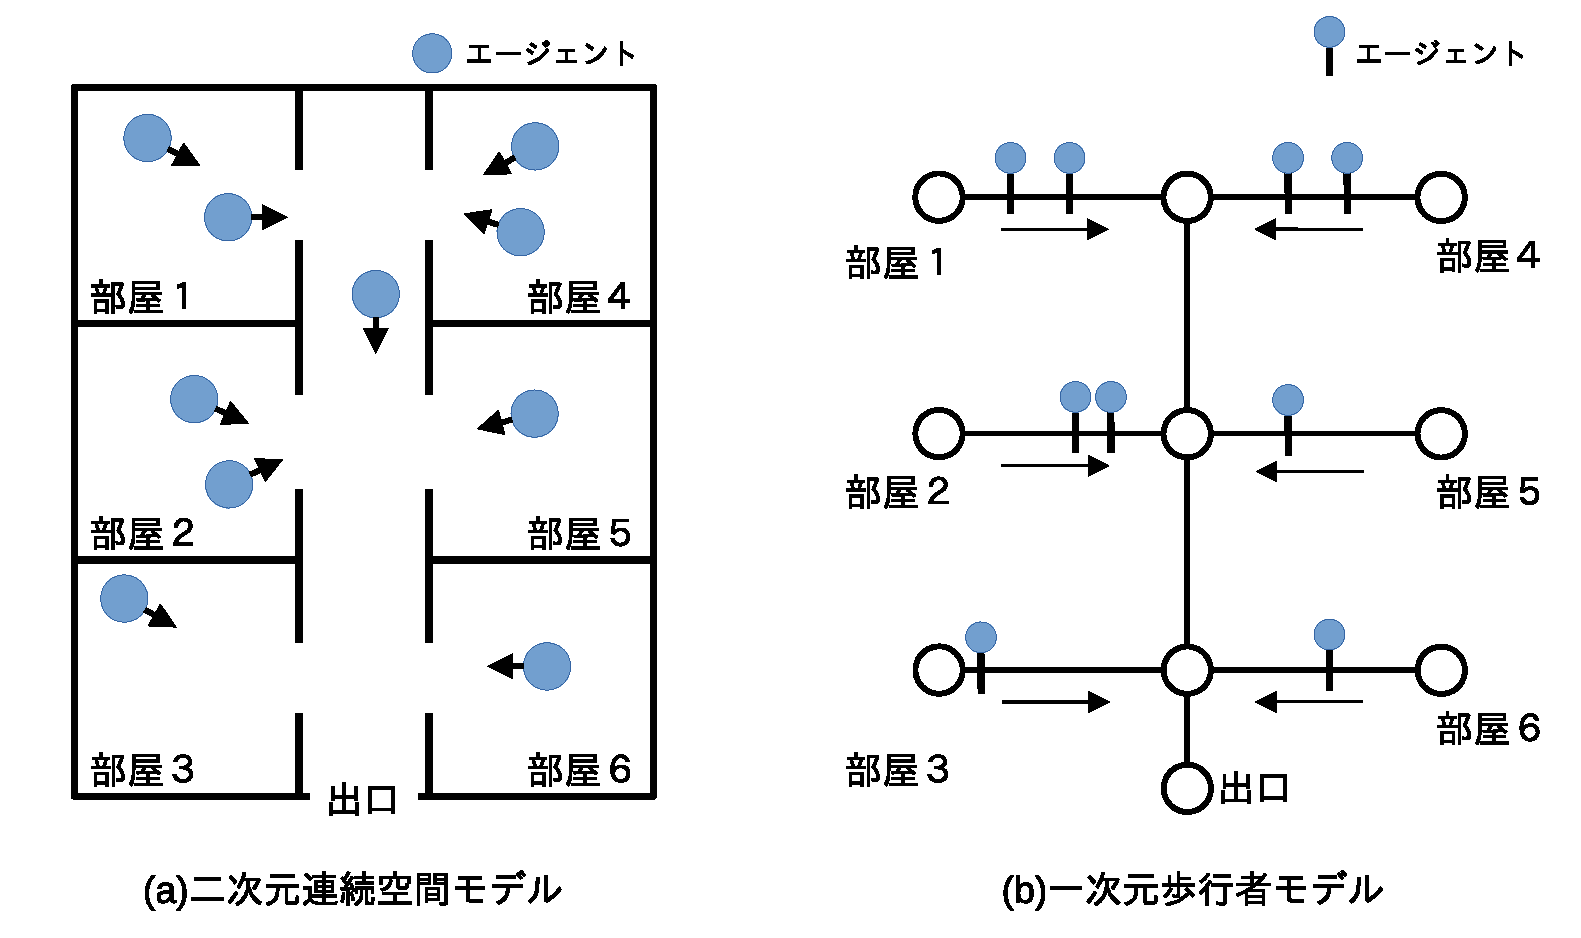
\includegraphics[width=11cm,clip]{figure/ichijigen_ex.eps}
  \caption{一次元モデルの例}
  \label{fig:ichijigen_ex}
 \end{center}
\end{figure}

\begin{figure}[hbtp]
 \begin{center}
  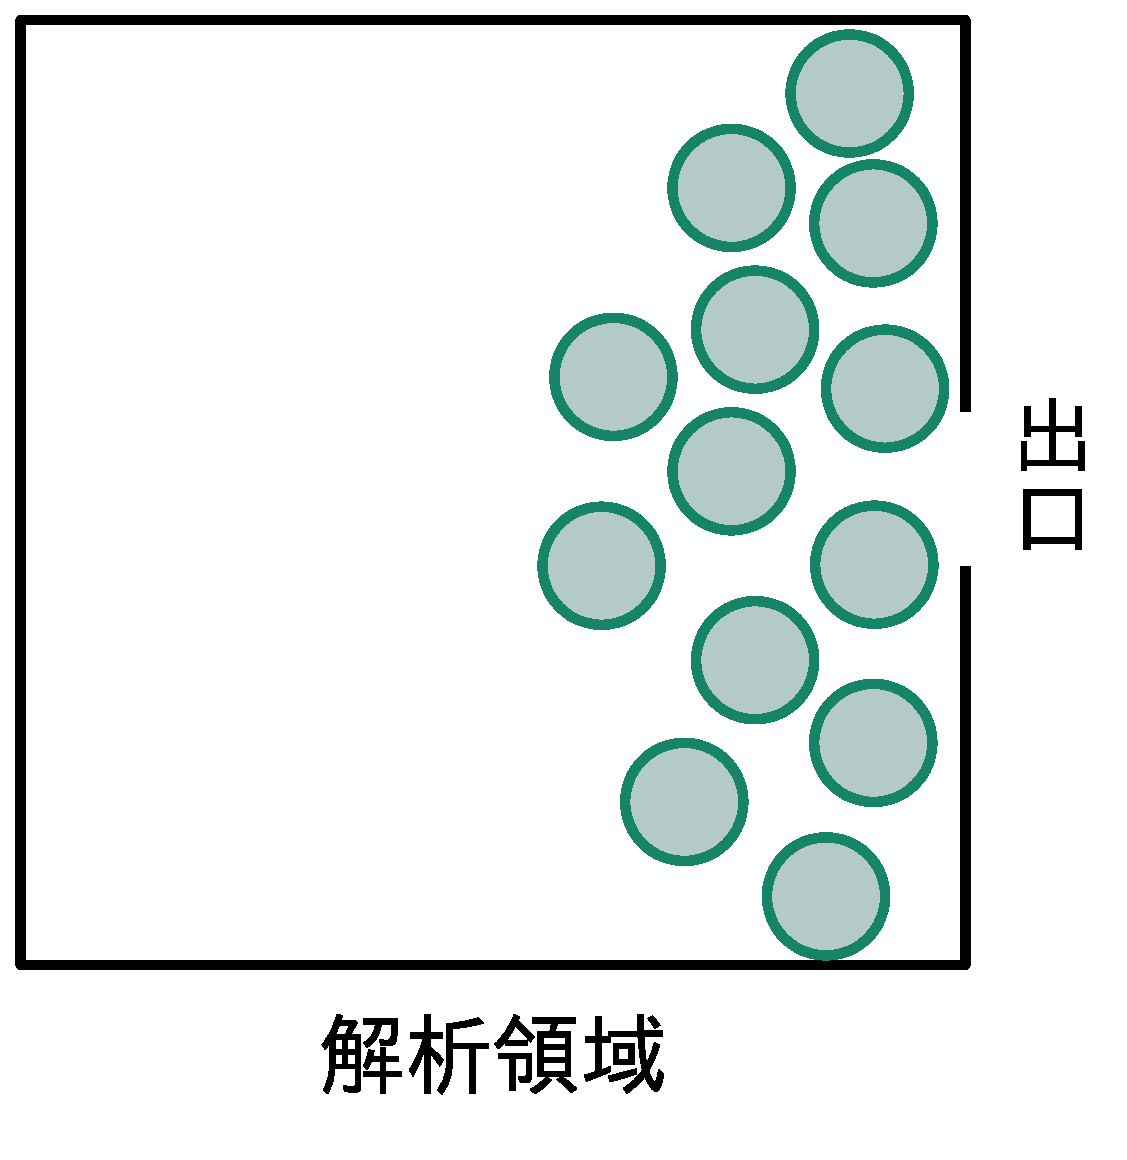
\includegraphics[width=4.5cm,clip]{figure/atigenshou.eps}
  \caption{アーチ現象の例}
  \label{fig:atigenshou}
 \end{center}
\end{figure}

\section{エージェント間の距離の計算回数削減}
SFMは,解析人数が増加するほど周囲のエージェントから受ける力の計算に
必要な周囲のエージェントが影響範囲内外かの判定の回数が増加する.
周囲のエージェントが影響範囲内外かの判定は,ルートなどを用いて
エージェント間距離$d_{ij}$を求める必要があるため,
特にエージェント間距離$d_{ij}$の計算に時間がかかる.
このため,SFMを用いた人流シミュレーションの解析時間を削減するためには,
エージェント間距離$d_{ij}$の計算回数を削減することが有効である.
エージェント間距離の計算回数削減手法にセル分割法や視野パラメータを用いた
削減手法がある.

\begin{figure}[t]
 \begin{center}
  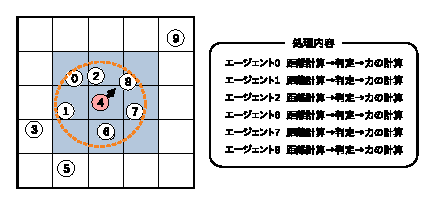
\includegraphics[width=11.5cm,clip]{figure/serubunkatu_ex1.eps}
  \caption{セル分割法を用いた例}
  \label{fig:seru_ex1}
 \end{center}
\end{figure}


\subsection{セル分割法}
セル分割法は,水や空気などの動きを解析できるMPS法\cite{mps}や銀河系などの圧縮性
流体に用いられるSPH法\cite{sph}などの粒子法によく用いられている.
粒子法は,近傍の粒子と相互作用する
力を計算し,粒子の行動を決定する.このため,セル分割法は,粒子法と同じように近傍の
エージェントとの相互作用力を計算するSFMに対しても用いられる.
本手法は,解析領域を格子上のセルに分割し,計算するエージェントの存在する
セルと近傍のセルに存在するエージェントに対して他のエージェントから受ける力の範囲であるか
判定し,範囲内であれば他のエージェントから受ける力を計算する手法である.
図\ref{fig:seru_ex1}にセル分割法を用いるSFMの例を示
す.図\ref{fig:seru_ex1}中の赤丸は他のエージェントから受ける力の計算をするエージ
ェント,黒丸は他のエージェント,四角は解析領域を格子状に分割したセルである.
この例では,エージェント4の行動を更新する際に青色のセル内に存在するエージェント
のみを参照するため,エージェント番号3,5,9の計算を削減できる.このとき,
視野を用いるSFMは,速度計算するエージェントの進行方向前方に存在するエージェント情報を
用いて計算するため,エージェントの進行方向後方のセルに存在するエージェント情報は不要になる,
このため,視野を用いるSFMでは,視野を考慮し,参照するセルを視野範囲に近づけることで,
計算回数を減らすことができる.
セル分割法の実装方法は,連結リスト法やハッシュ法などがよく用いられる(参考文献).

連結リスト法は,単方向リストを用いたセル分割法である.
\figref{fig:renketu_list}に連結リスト法を用いたセル分割法の例を示す.
\figref{fig:renketu_list}中の左側にある四角は解析領域,解析領域内の格子はセル分割法の
格子,各格子内の左下に記された番号は格子の番号,白色の丸はエージェント,
丸の中の番号は,エージェント番号を示す.また,図中の左側は,連結リスト法のデータ構造を
示しており,青色の四角は各格子の先頭,緑色の四角はエージェントのノードを示す.
\figref{fig:renketu_list}のように,各エージェントは,同じ格子に存在する他のエージェントの
インデックス番号を保持することで,単方向のリストを作成する.
各格子内の最後のエージェントは,最後のエージェントを示す-1を保持する.
周囲のエージェントを参照するときは,周囲のセルの先頭から終端のエージェントを
辿ることで,周囲のセルに存在するエージェントを
絞ることができる.

\begin{figure}[t]
 \begin{center}
  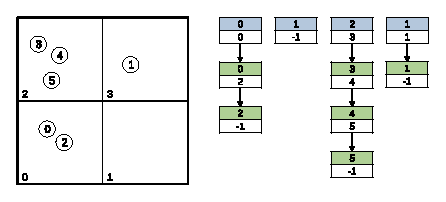
\includegraphics[width=11.5cm,clip]{figure/serubunkatu_serurinku.eps}
  \caption{連結リスト法を用いたセル分割法の例}
  \label{fig:renketu_list}
 \end{center}
\end{figure}

\begin{figure}[t]
 \begin{center}
  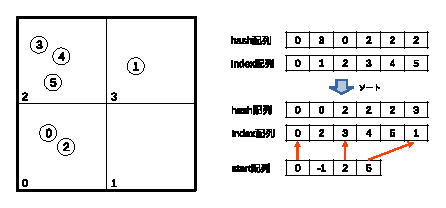
\includegraphics[width=11.5cm,clip]{figure/serubunkatu_hash.eps}
  \caption{ハッシュを用いたセル分割法の例}
  \label{fig:hash}
 \end{center}
\end{figure}

ハッシュ法は,3つの配列を用いてセル分割法を実装する方法である.
ハッシュ法の配列は,hash配列とindex配列,start配列の3つで構成される.
hash配列は,エージェントの所属するセルの番号を保持する.また,index配列は,
エージェントのインデックス番号を保持する.start配列は,各セルの始点を示すインデックス
を保持する.
\figref{fig:hash}にハッシュ法を用いたセル分割法を示す.
\figref{fig:hash}中の右側に示す四角は,各配列を示す.
\figref{fig:hash}に示すように,ハッシュ法は,index配列に各エージェントの
インデックス番号,hash配列に各エージェントのセル番号を格納する.次に,
hash配列とindex配列をhash配列の値を用いて昇順にソートを行う.
ソート後は,start配列に各セルのhash配列の始点を格納する.
エージェントが存在しないセルは,hash配列の値に-1を格納する.
周囲のエージェントを参照するときは,start配列から参照するセルの
始点を取得し,hash配列のセル番号が変わるまで繰り返すことで,
周囲のエージェントを絞ることができる.


\begin{figure}[t]
 \begin{center}
  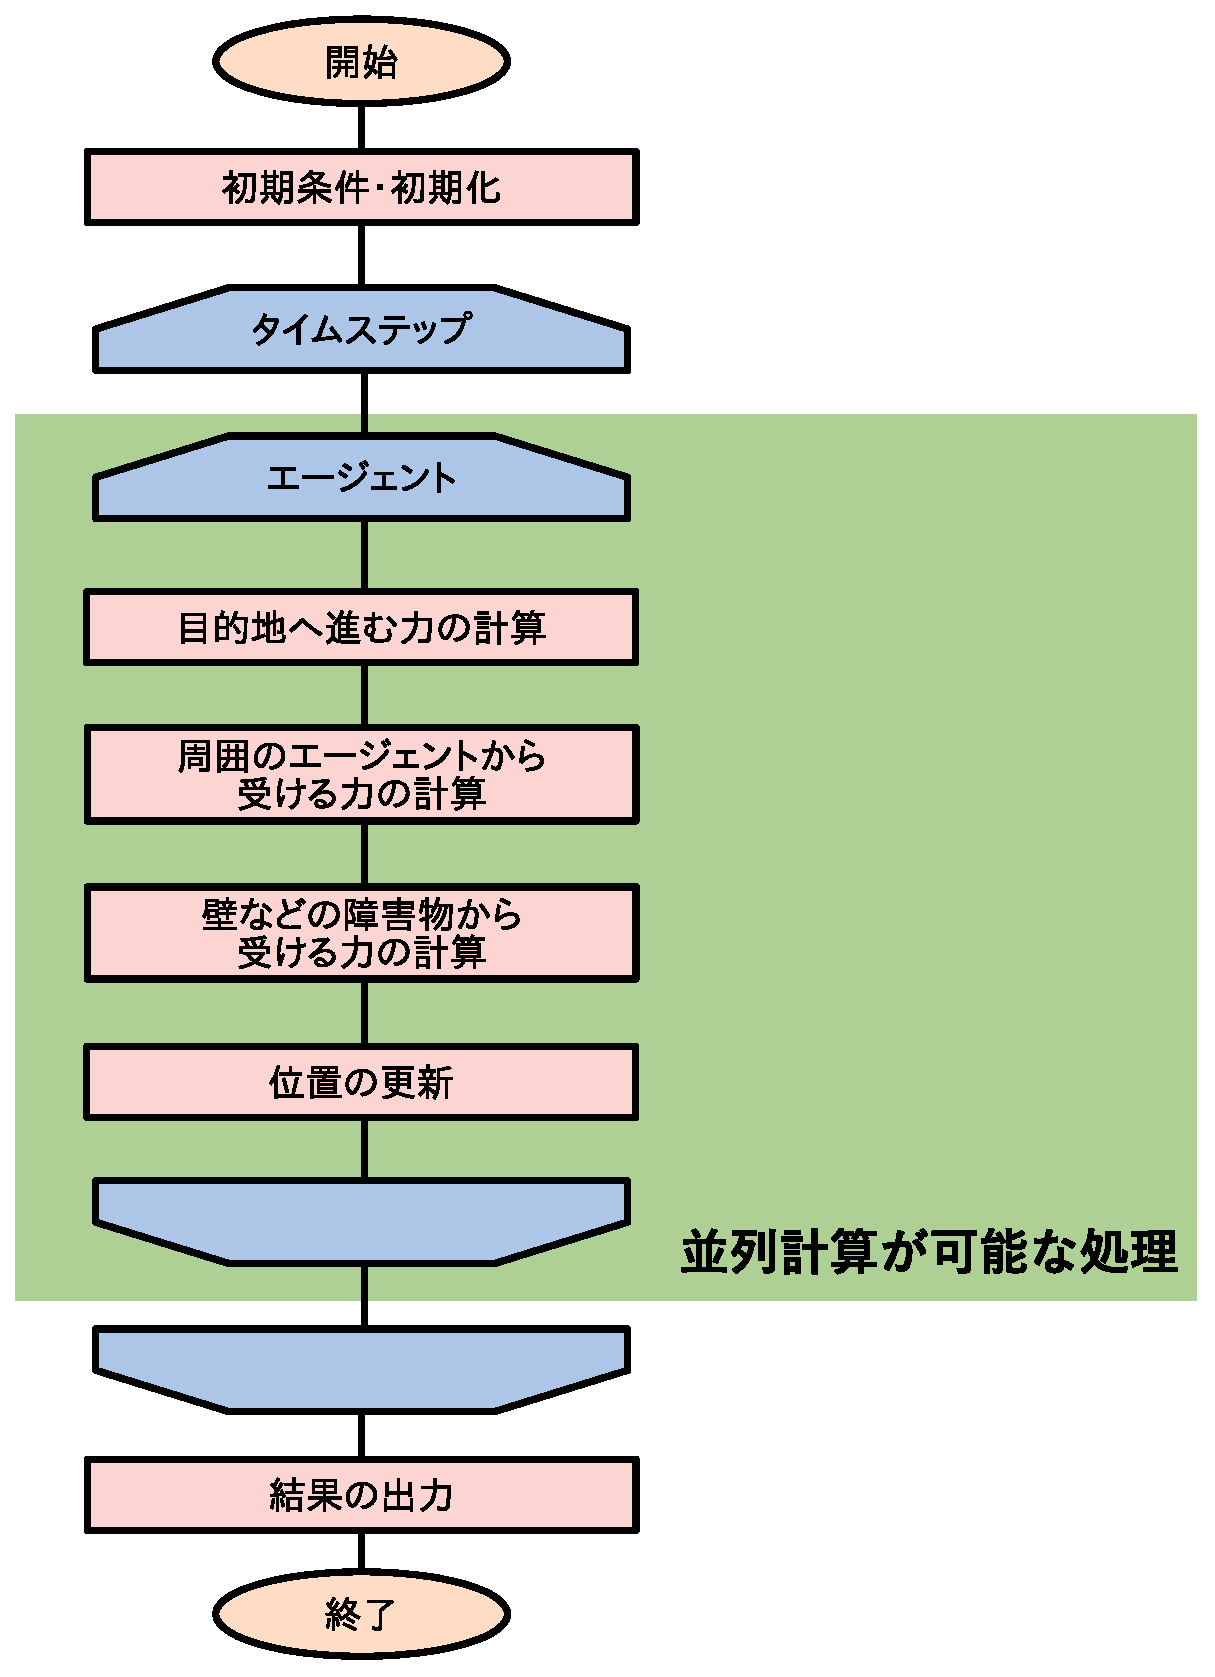
\includegraphics[width=8cm,clip]{figure/heiretuka_sfm.eps}
  \caption{SFMの並列化可能な処理}
  \label{fig:sfm_heiretu}
 \end{center}
\end{figure}

\section{単位時間あたりの計算回数を多くする手法}
SFMは,エージェントごとの計算に並列性があるため,
高い並列性を得ることが可能である.
\figref{fig:sfm_heiretu}にSFMの並列に計算できる処理を示したフローチャートを示す.
\figref{fig:sfm_heiretu}中の緑色の四角は並列計算が可能な処理である.
\figref{fig:sfm_heiretu}に示すように,SFMは,エージェントごとの進行方向を決定するための
計算を並列に処理することができる.
SFMを並列に実行するためには,GPU(Graphics Processing Unit)やMPI(Messaage Passing Intereface)
を用いた手法が用いられている.
GPUを用いたSFMは,エージェントごとの計算をスレッドごとに並列に計算する方法が
一般的である\cite{seru_sfm1}\cite{seru_sfm2}.
\figref{fig:agent_heiretu}に3スレッドで並列化したSFMの例を示す.
\figref{fig:agent_heiretu}中の緑色の丸はスレッド1が計算するエージェント,
赤色の丸はスレッド2が計算するエージェント,
青色の丸はスレッド3が計算するエージェントである.
\figref{fig:agent_heiretu}に示すように,GPUなどを用いた並列化手法は,
それぞれのスレッドが担当するエージェント数が等しくなるように,
各スレッドで分割し,エージェントの進行方向を計算する.
MPIを用いた並列化手法は,主に分散メモリ環境に用いられているため,
各プロセッサ間の通信時間が余計に時間がかかる.
このため,MPIを用いたSFMでは,各プロセッサ間の通信回数を削減するために,
各プロセッサの担当するエージェントを解析領域ごとに決定することが一般的である.
\figref{fig:ryouiki_heiretu}にMPIを用いたSFMの領域分割の例を示す.
\figref{fig:ryouiki_heiretu}中の
黄色の丸はプロセッサ(PE)1が担当するエージェント,
赤色の丸はPE2が担当するエージェント,
青色の丸はPE3が担当するエージェント,
緑色の丸はPE4が担当するエージェントである.
\figref{fig:ryouiki_heiretu}のように,MPIを用いたSFMは,
各PEに担当する領域に存在するエージェントの進行方向を計算する.

\begin{figure}[t]
 \begin{center}
  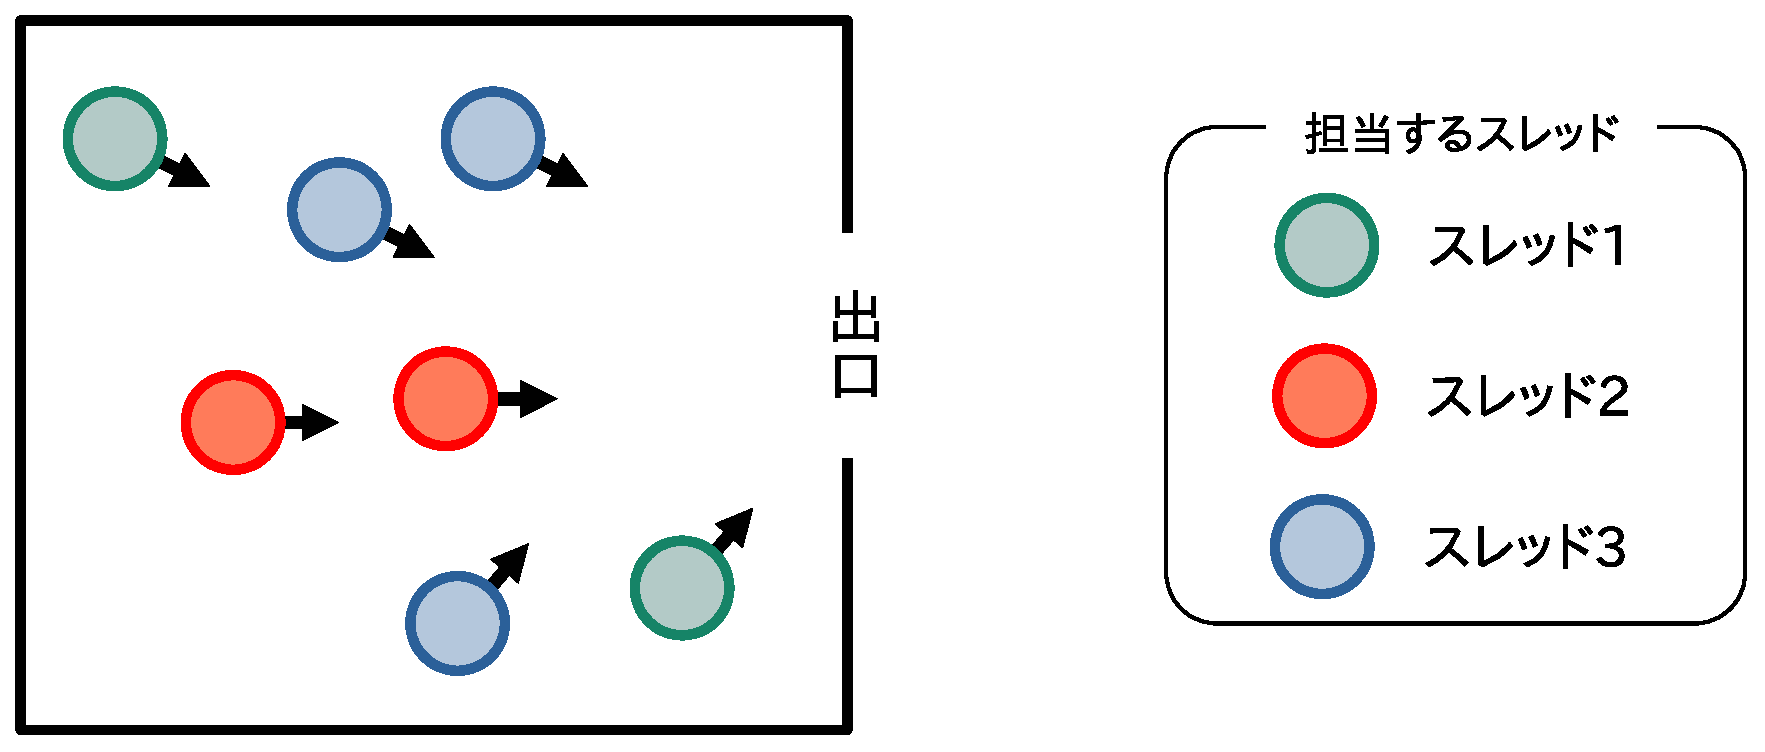
\includegraphics[width=10cm,clip]{figure/sureddo_heiretu.eps}
  \caption{3スレッドでの並列化の例}
  \label{fig:agent_heiretu}
 \end{center}
\end{figure}

\begin{figure}[t]
 \begin{center}
  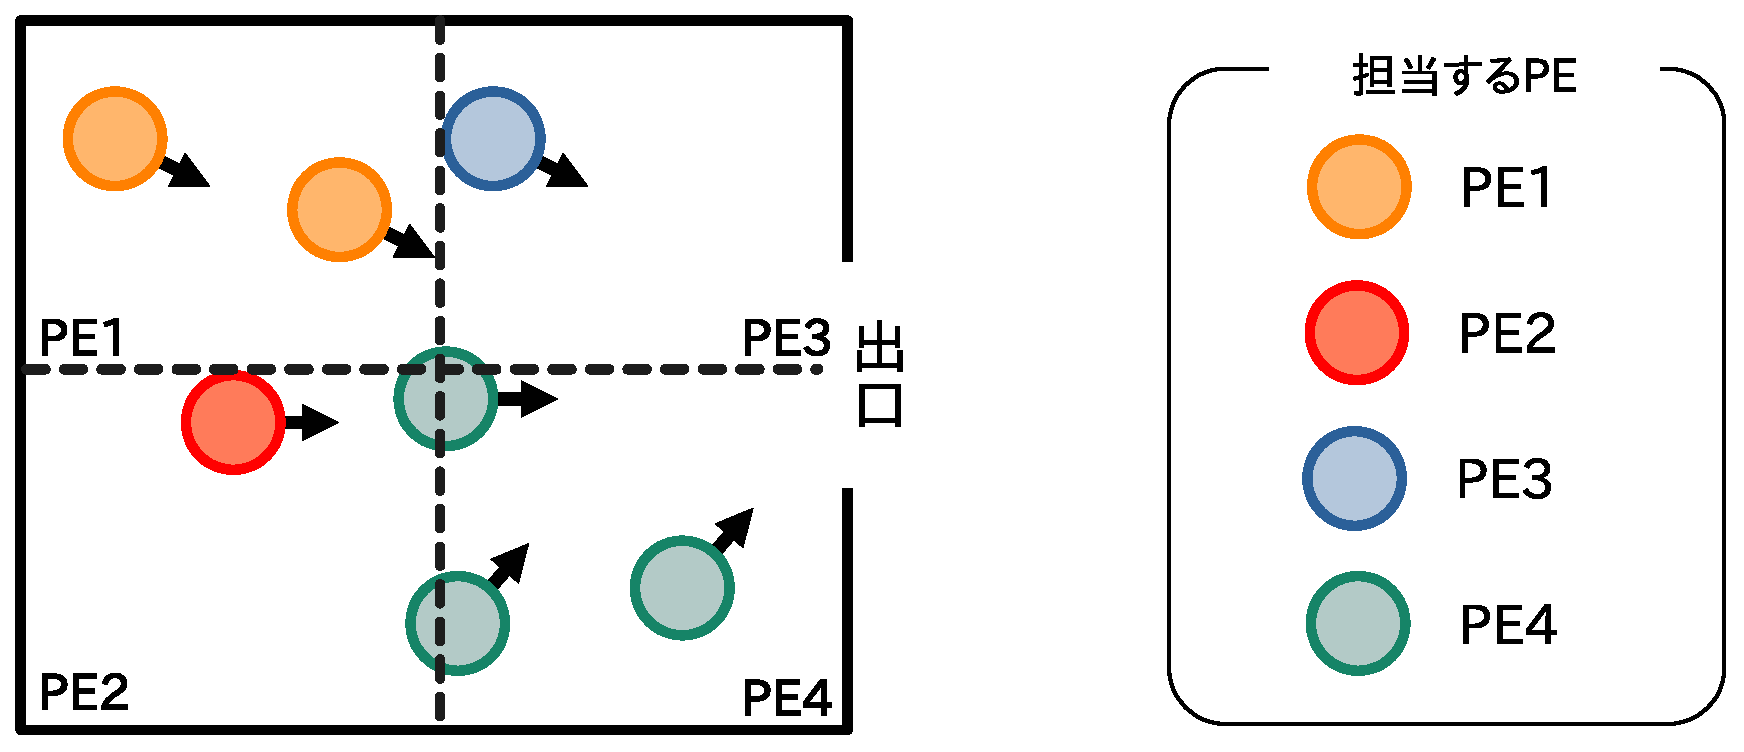
\includegraphics[width=10cm,clip]{figure/ryoiki_heiretu.eps}
  \caption{MPIを用いたSFMの領域分割の例}
  \label{fig:ryouiki_heiretu}
 \end{center}
\end{figure}

\clearpage
\section{経路選択の判定回数削減(工事中)}
SFMを用いた避難シミュレーションでは,エージェントが出口までに
避難できるようにダイクストラ法などを用いて次に進む経由地を決定する.
避難シミュレーションは,火災や震災などの被害状況に応じて避難経路が
変わるため,解析中に何度も経路を決定する判定が必要になる.
経路選択の判定は,ダイクストラ法などのグラフ理論に用いられる手法を使用するため,
経由地数が多くなるほど判定に時間がかかる.
このため,経路選択の判定回数を削減する手法に,経路グラフの簡易化や,
〇〇の手法が提案されている.

経由地グラフの簡易化は,解析する規模が大きくなるほど,経由地数が多くなるため,


%***** END ************************************************
